% !TEX program = pdflatex
% ============================================================
%  COMPETITION RULES — UAV CONTEST 2027
%  The 4th International Competition on Research and Design
%  of Unmanned Aerial Vehicles — Ton Duc Thang University
%  Official Rules Document — All Technical Specifications Approved
% ============================================================
\documentclass[12pt,a4paper]{article}

\usepackage[utf8]{inputenc}
\usepackage[T1]{fontenc}
\usepackage{mathptmx}
\usepackage{geometry}
\geometry{a4paper, margin=2.4cm}
\usepackage{booktabs}
\usepackage{multirow}
\usepackage{longtable}
\usepackage{array}
\usepackage{enumitem}
\usepackage{xcolor}
\usepackage{tikz}
\usetikzlibrary{positioning, calc, arrows.meta}
\usepackage{fancyhdr}
\usepackage{titlesec}
\usepackage{hyperref}
\usepackage{amsmath}
\usepackage{amssymb}
\usepackage{colortbl}

\hypersetup{
    colorlinks=true,
    linkcolor=blue!50!black,
    urlcolor=blue!50!black,
    pdftitle={UAV Contest 2027 - Official Competition Rules},
    pdfauthor={Organizing Committee, UAV Contest, Ton Duc Thang University}
}

\renewcommand{\thesection}{\Roman{section}}
\titleformat{\section}{\normalfont\Large\bfseries}{\thesection.}{0.6em}{}
\titleformat{\subsection}{\normalfont\large\bfseries}{\thesubsection}{0.6em}{}

\pagestyle{fancy}
\setlength{\headheight}{14pt}
\fancyhf{}
\fancyhead[L]{\small UAV Contest 2027 — Competition Rules (Official)}
\fancyhead[R]{\small Issued: September 2026}
\fancyfoot[C]{\thepage}
\renewcommand{\headrulewidth}{0.4pt}

\definecolor{depotgreen}{RGB}{46,139,87}
\definecolor{pickupyellowbg}{RGB}{255,243,205}
\definecolor{redpt}{RGB}{252,42,27}
\definecolor{yellowpt}{RGB}{250,255,55}
\definecolor{bluept}{RGB}{60,0,251}
\definecolor{approvedgreen}{RGB}{0,128,0}
\definecolor{headerblue}{RGB}{31,78,120}

\newcommand{\approved}[1]{\textcolor{approvedgreen}{\textbf{[APPROVED: #1]}}}
\newcommand{\newmark}{\textcolor{headerblue}{\textbf{[NEW]}}}

\setlist[itemize]{leftmargin=1.6em}
\setlist[enumerate]{leftmargin=1.8em}

\begin{document}

% ============================================================
\begin{titlepage}
\centering
\vspace*{1.2cm}
{\Large\bfseries TON DUC THANG UNIVERSITY}\\[0.2cm]
{\large FACULTY OF ELECTRICAL — ELECTRONICS ENGINEERING \& CPAS LAB}\\[1.6cm]

{\Huge\bfseries OFFICIAL COMPETITION RULES}\\[0.4cm]
{\Large\bfseries UAV CONTEST 2027}\\[0.6cm]
{\large The 4th International Competition on Research}\\
{\large and Design of Unmanned Aerial Vehicles}\\[0.6cm]
{\large Celebrating the 30th Anniversary of Ton Duc Thang University (1997 -- 2027)}\\[0.3cm]
{\large Official Competition Dates: \textbf{September 20 and 21, 2027}}\\[0.3cm]
{\normalsize Venue: Multi-Purpose Sports Arena, Tan Phong Main Campus, Ho Chi Minh City}\\[2.0cm]

{\large\bfseries Theme: AUTONOMOUS LOW-ALTITUDE LOGISTICS ECOSYSTEM}\\[2.5cm]

{\normalsize Version: \textbf{Official Rules (Fully Approved)}}\\[0.3cm]
{\normalsize All technical parameters and operational criteria officially finalized}\\[2cm]

\vfill
{\small Official competition standard issued by the Organizing Committee (BOC) of UAV Contest. Applicable to all participating teams competing on September 20 and 21, 2027.}
\end{titlepage}

\tableofcontents
\newpage

% ============================================================
\section{PURPOSE AND CONTEXT}

The low-altitude economy and autonomous logistics are emerging as a strategic digital infrastructure pillar within national science, technology, and innovation development priorities according to Prime Minister Decision No. 808/QD-TTg. Unlike traditional emergency-response scenarios — where a single unmanned aerial vehicle (UAV) operates independently to complete one discrete mission — real-world low-altitude logistics infrastructure operates on a fundamentally different principle: multiple agents (UAVs, ground robots, transfer stations) share the same physical space and must coordinate safely and efficiently, without necessarily relying on a single real-time central controller.

UAV Contest 2027 simulates an \textbf{Autonomous Low-Altitude Logistics Distribution Hub}. Each participating team operates a self-built UAV to execute a chain of missions: retrieving packages from a source location, transporting them, and delivering them with precision to a destination point — including a destination that is itself in motion. The competition is organized into three rounds (Preliminary, Semi-Final, and Final) with progressively increasing difficulty and autonomy requirements, alongside a voluntary category — \textbf{Coordinated Ops} — which evaluates the ability of two UAVs to coordinate through the standardized CPAS Agent Beacon Protocol (CABP).

% ============================================================
\section{COMPETITION OBJECTIVES}

\begin{itemize}
\item \textbf{Practical Application:} Developing and optimizing the deployment of UAVs for low-altitude logistics operations — retrieval, transport, and precision delivery within a realistic simulated environment.
\item \textbf{Innovation and Creativity:} Fostering innovation in airframe mechanics, embedded electronics integration, and advanced flight control under GPS-denied environments.
\item \textbf{Comprehensive Evaluation:} Concurrently assessing manual piloting skills, fully autonomous capabilities (Edge AI and computer vision), and multi-agent coordination between two UAVs sharing the same physical airspace.
\end{itemize}

% ============================================================
\section{UAV TECHNICAL SPECIFICATIONS}

\subsection*{1. General Configuration}
\begin{itemize}
\item \textbf{Maximum Dimensions:} $1.0 \times 1.0 \times 1.0$ meters (inclusive of propellers and propeller guards).
\item \textbf{Maximum Takeoff Weight (MTOW):} $\leq 5.0$ kg (including batteries and all onboard mission payloads).
\item \textbf{Power System:}
  \begin{itemize}
    \item Battery Type: LiPo/Li-ion, maximum 6S configuration.
    \item Quantity: maximum 3 battery packs mounted on the airframe.
    \item Total Energy Capacity: $\leq 300$ Wh.
  \end{itemize}
\item \textbf{Payload Capacity:} The UAV is permitted to carry up to five (05) package simulants upon takeoff for the autonomous delivery phase. Packages must be pre-loaded prior to match commencement.
\item \textbf{System Integrity:} Electrical and mechanical assemblies must maintain high safety standards with zero risk of leakage, short circuits, or thermal runaway.
\end{itemize}

\subsection*{2. Mandatory Safety Requirements}
\begin{itemize}
\item \textbf{Propeller Guards:} 100\% mandatory installation of protective guards/shrouds for all propellers.
\item \textbf{Manual Override:} Emergency manual control takeover capability must be readily available at all times.
\item \textbf{Fail-Safe Mechanism:} Automatic activation of Return-to-Home (RTH) or emergency landing upon loss of RC/Telemetry signal exceeding 3 seconds or on critical battery.
\item \textbf{Status Indicators:} LED status indicators (strongly encouraged).
\item \textbf{Personnel Safety:} Physical design must present no sharp hazards to operators or referees.
\item \textbf{Laser Radiation:} Non-ionizing laser systems must comply with IEC 60825-1 (Class 2 / 2M maximum). Ionizing radiation is strictly prohibited.
\end{itemize}

\subsection*{3. Control Systems}
\begin{itemize}
\item \textbf{Phase 1 — Pickup:} Manual or semi-autonomous flight control permitted.
\item \textbf{Phase 2 — Delivery:} Fully autonomous flight via waypoints or onboard computer vision. Manual intervention is strictly prohibited, except in emergency situations verified by referees.
\item \textbf{Coordinated Ops Track:} Both UAVs must continuously broadcast standardized CABP messages at $\geq 5\text{ Hz}$ throughout the entire flight duration.
\end{itemize}

\subsection*{4. Radio Communication and Localization Equipment}
\begin{itemize}
\item \textbf{Regulatory Compliance:} All radio transmission equipment must strictly comply with Vietnam's Radio Frequency Law.
\item \textbf{Prohibited Placement:} Placing radio positioning devices (anchors, beacons) directly on the arena playing surface (Playfield) is strictly prohibited.
\item \textbf{External UWB Permitted:} Positioning systems utilizing anchors located in the perimeter zone outside the playfield (e.g., UWB RTLS) are fully permitted.
\item \textbf{Signal Disclaimer:} The BOC provides dedicated Wi-Fi channels per team but strongly recommends that teams design backup plans for RF interference.
\end{itemize}

\subsection*{5. Package Handling Mechanisms}
\begin{itemize}
\item \textbf{Gripping Mechanism:} Must not damage the structural integrity of large package models. Minimum lifting capacity $\geq 300$g. Must feature a safety locking mechanism preventing unintentional release during flight.
\item \textbf{Dispensing Mechanism:} Capable of dispensing individual packages with precision. Minimum capacity of 05 packages at takeoff. During dispensing, the lowest point of the UAV must maintain an altitude $\geq 3.0$ meters above the floor.
\end{itemize}

\subsection*{6. Standardized Competition Materials}
\begin{itemize}
\item \textbf{Package Simulants (Small):} Standardized to regulation tennis balls, diameter $65.41$–$68.58$ mm, mass $56.0$–$59.4$ g, delivered into Delivery Points D1–D5.
\item \textbf{Large Package Models:} Rigid cubic block $0.3 \times 0.3 \times 0.3$ meters, mass $300$ grams, equipped with an integrated handle or hook for gripping.
\end{itemize}

% ============================================================
\section{ARENA SPECIFICATIONS}

\begin{itemize}
\item \textbf{Overall Dimensions:} $12.0 \times 24.0$ meters.
\item \textbf{Depot (Safe Zone):} $12.0 \times 3.5$ meters — houses takeoff/landing pads and mission dispatch/arrival stations.
\item \textbf{Air Corridor Checkpoints (ACC1 to ACC4):} Inner ring diameter $1.6$ meters; center height $1.7$ meters; total structure height $2.6$ meters. ACC1–ACC2 serve the outbound path; ACC3–ACC4 serve the return path.
\item \textbf{Pickup Area:} $12.0 \times 4.5$ meters. Stations P1, P2, P3 have platform dimensions $1.0 \times 1.0$ meters at an elevation of $1.0$ meter above the floor.
\item \textbf{Delivery Points (D1 to D5):} Positioned $0.1$ meters above the floor, equipped with integrated sensors for automatic score validation.
\item \textbf{Operational Altitude Limits:} Manual flight $\leq 5.0$ meters; Autonomous flight $3.0$–$5.0$ meters.
\item \textbf{Mobile Receiver (Final Round only):} Moves linearly back-and-forth at a constant velocity of \textbf{$10$ cm/s} along a fixed guide rail.
\end{itemize}

\begin{figure}[h]
\centering
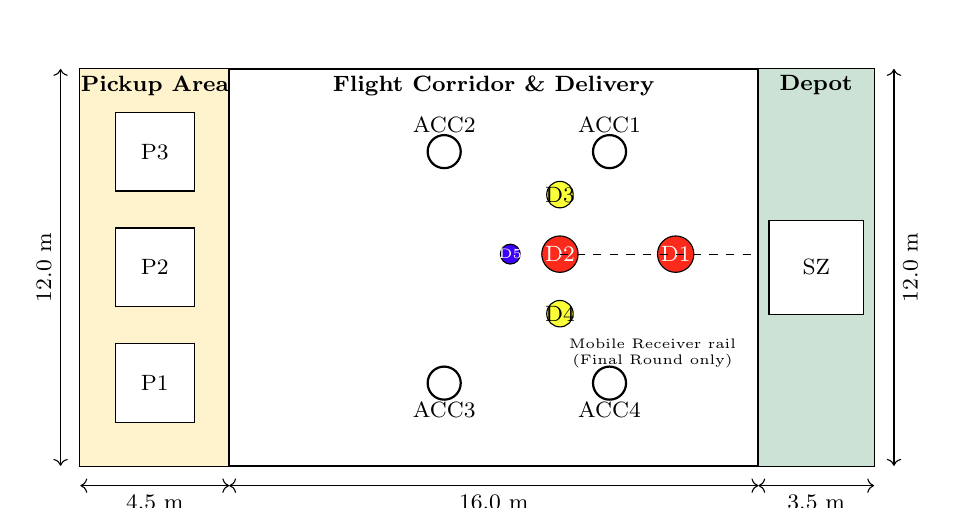
\begin{tikzpicture}[scale=0.42, every node/.style={font=\footnotesize}]
  % Overall arena outline
  \draw[thick] (0,0) rectangle (24,12);

  % Pickup Area
  \fill[pickupyellowbg] (0,0) rectangle (4.5,12);
  \draw[thick] (4.5,0) -- (4.5,12);
  \node[align=center] at (2.25,11.5) {\textbf{Pickup Area}};
  \node[draw, fill=white, minimum width=1cm, minimum height=1cm] (P1) at (2.25,2.5) {P1};
  \node[draw, fill=white, minimum width=1cm, minimum height=1cm] (P2) at (2.25,6.0) {P2};
  \node[draw, fill=white, minimum width=1cm, minimum height=1cm] (P3) at (2.25,9.5) {P3};

  % Depot
  \fill[depotgreen!25] (20.5,0) rectangle (24,12);
  \draw[thick] (20.5,0) -- (20.5,12);
  \node at (22.25,11.5) {\textbf{Depot}};
  \node[draw, fill=white, minimum width=1.2cm, minimum height=1.2cm] (SZ) at (22.25,6.0) {SZ};

  % Middle zone
  \node[align=center] at (12.5,11.5) {\textbf{Flight Corridor \& Delivery}};

  % ACC gates
  \draw[thick] (16,9.5) circle (0.5); \node at (16,10.3) {ACC1};
  \draw[thick] (11,9.5) circle (0.5); \node at (11,10.3) {ACC2};
  \draw[thick] (16,2.5) circle (0.5); \node at (16,1.7) {ACC4};
  \draw[thick] (11,2.5) circle (0.5); \node at (11,1.7) {ACC3};

  % Delivery points D1..D5
  \draw[fill=redpt] (18,6.4) circle (0.55); \node[white] at (18,6.4) {D1};
  \draw[fill=redpt] (14.5,6.4) circle (0.55); \node[white] at (14.5,6.4) {D2};
  \draw[fill=yellowpt] (14.5,8.2) circle (0.4); \node at (14.5,8.2) {D3};
  \draw[fill=yellowpt] (14.5,4.6) circle (0.4); \node at (14.5,4.6) {D4};
  \draw[fill=bluept] (13.0,6.4) circle (0.3); \node[white] at (13.0,6.4) {\tiny D5};

  % Mobile receiver rail
  \draw[dashed] (14.5,6.4) -- (20.5,6.4);
  \node[align=center, font=\tiny] at (17.3,3.4) {Mobile Receiver rail\\(Final Round only)};

  % Dimension annotations
  \draw[<->] (0,-0.6) -- (4.5,-0.6); \node at (2.25,-1.1) {4.5 m};
  \draw[<->] (4.5,-0.6) -- (20.5,-0.6); \node at (12.5,-1.1) {16.0 m};
  \draw[<->] (20.5,-0.6) -- (24,-0.6); \node at (22.25,-1.1) {3.5 m};
  \draw[<->] (-0.6,0) -- (-0.6,12); \node[rotate=90] at (-1.1,6) {12.0 m};
  \draw[<->] (24.6,0) -- (24.6,12); \node[rotate=90] at (25.1,6) {12.0 m};
\end{tikzpicture}
\caption{Arena layout schematic ($12 \times 24$ m). D1,D2: Red ($\varnothing$1.0m); D3,D4: Yellow ($\varnothing$0.6m); D5: Blue ($\varnothing$0.4m).}
\end{figure}

% ============================================================
\section{MISSION REQUIREMENTS}

\subsection*{A. PRELIMINARY ROUND}
\paragraph{Phase 1 — Pickup (Manual or Semi-Autonomous Control)}
\begin{enumerate}
\item \textbf{Takeoff and Approach:} UAV departs from Depot, passing cleanly through the center of ACC1 and ACC2.
\item \textbf{Pickup Execution:} UAV approaches P1, P2, or P3 and retrieves exactly one (01) large package model.
\item \textbf{Transport and Return:} UAV transports the package back through ACC3 and ACC4, placing it safely into the Depot.
\item \textbf{Landing:} Controlled landing at the designated pad.
\end{enumerate}

\paragraph{Phase 2 — Delivery (100\% Autonomous Flight)}
\begin{itemize}
\item \textbf{Mission 1 — Autonomous Takeoff:} Autonomous mode engaged; UAV climbs to an altitude $\geq 3.0$ meters without RC intervention.
\item \textbf{Mission 2 — Precision Delivery:} UAV navigates to D1–D5 and dispenses package simulants into target rings. In the Preliminary Round, target coordinates are \textbf{FIXED}. Each point scores only upon the first valid drop.
\item \textbf{Mission 3 — Autonomous Precision Landing:} UAV autonomously returns to Depot, performs a precision landing, and disarms motors.
\end{itemize}

\subsection*{B. SEMI-FINAL ROUND}
\begin{itemize}
\item Phase 1 procedure is identical to the Preliminary Round.
\item Phase 2: Coordinates for D1–D5 are \textbf{NOT FIXED}. The Referee Panel conducts a random draw from the position matrix prior to each match. UAVs must use onboard computer vision to identify targets.
\end{itemize}

\subsection*{C. FINAL ROUND}
\begin{itemize}
\item Phase 1 procedure is identical to the Preliminary Round.
\item Phase 2: Coordinates for D1–D5 are drawn randomly. \textbf{Target D2 is mounted on the Mobile Receiver}, moving at a constant speed of $10$ cm/s along a fixed linear guide path.
\end{itemize}

\subsection*{D. VOLUNTARY TRACK: COORDINATED OPS — "PLACE — RELAY — RETRIEVE"}

Applies to teams operating \textbf{two UAVs}: \textbf{UAV-A} (manual/semi-autonomous) and \textbf{UAV-B} (fully autonomous) in a sequential relay chain:

\paragraph{Operational Rules and Validation}
\begin{itemize}
\item \textbf{Voluntary Participation:} Independent bonus track. Teams failing or opting out retain $100\%$ of their standard-track score.
\item \textbf{Candidate Draw:} The Referee Panel draws a candidate subset of exactly \textbf{03 out of 05 D-points} (a 3/5 subset of D1–D5).
\item \textbf{Code Integrity Checksum:} Teams submit the \textbf{SHA-256 checksum} and software file copy for UAV-B to the Technical Committee at least 30 minutes prior to the draw.
\item \textbf{Standardized QR Codes:} Each point D carries a standard \textbf{$15 \times 15$ cm} QR code affixed at its center.
\end{itemize}

\paragraph{Phase 1 — Placement (UAV-A)}
Within time window \textbf{$T_1 = 90$ seconds}, UAV-A places 01 package accurately at one of the 3 candidate points. Upon placement, UAV-A transmits the `mission\_event` message via CABP.

\paragraph{Phase 2 — Retrieval (UAV-B)}
Within time window \textbf{$T_2 = 120$ seconds}, measured from Phase 1 completion:
\begin{itemize}
\item \textbf{Bonus Path (CABP Successful):} If UAV-B receives a valid `mission\_event` within the timeout threshold of \textbf{$3.0$ seconds}, it skips sequential scanning and flies directly to the destination point.
\item \textbf{Baseline Path (Automatic Fallback):} If 3.0 seconds elapse without receiving a valid message, UAV-B \textbf{automatically initiates} sequential scanning of candidate points via QR code verification and executes retrieval.
\end{itemize}

\paragraph{Total Match Duration for Coordinated Ops}
Officially finalized at \textbf{07 minutes} (compared to 5 minutes for the standard track).

% ============================================================
\section{SCORING CRITERIA}

\subsection*{A. Preliminary and Semi-Final Rounds Scoring}
\begin{longtable}{p{3.0cm}p{6.0cm}p{3.8cm}p{1.6cm}}
\toprule
\textbf{Category} & \textbf{Mission Details} & \textbf{Scoring Criteria} & \textbf{Max. Score} \\
\midrule
\endfirsthead
\toprule
\textbf{Category} & \textbf{Mission Details} & \textbf{Scoring Criteria} & \textbf{Max. Score} \\
\midrule
\endhead
\multirow{3}{3.0cm}{Phase 1: Pickup} & Air Corridor Checkpoints (ACC1–ACC4) & 5 points per checkpoint & 20 \\
 & Successful retrieval and return to Depot & 20 points per package (P1–P3) & 60 \\
 & Precision landing & 10 points & 10 \\
\midrule
\multicolumn{3}{r}{\textbf{Phase 1 Total}} & \textbf{90} \\
\midrule
\multirow{5}{3.0cm}{Phase 2: Delivery} & Autonomous takeoff (altitude $\geq 3.0$m) & 20 points & 20 \\
 & Delivery to D1, D2 (Red, $\varnothing$1.0m) & 20 points $\times$ 2 locations & 40 \\
 & Delivery to D3, D4 (Yellow, $\varnothing$0.6m) & 30 points $\times$ 2 locations & 60 \\
 & Delivery to D5 (Blue, $\varnothing$0.4m) & 50 points $\times$ 1 location & 50 \\
 & Autonomous precision landing at Depot & 30 points & 30 \\
\midrule
\multicolumn{3}{r}{\textbf{Phase 2 Total}} & \textbf{200} \\
\midrule
\multicolumn{3}{r}{\textbf{TOTAL STANDARD SCORE}} & \textbf{290} \\
\bottomrule
\end{longtable}

\subsection*{B. Final Round Scoring}
\begin{longtable}{p{3.0cm}p{6.0cm}p{3.8cm}p{1.6cm}}
\toprule
\textbf{Category} & \textbf{Mission Details} & \textbf{Scoring Criteria} & \textbf{Max. Score} \\
\midrule
\endfirsthead
\toprule
\textbf{Category} & \textbf{Mission Details} & \textbf{Scoring Criteria} & \textbf{Max. Score} \\
\midrule
\endhead
Phase 1: Pickup & (Identical structure to Preliminary Round) & & 90 \\
\midrule
\multirow{6}{3.0cm}{Phase 2: Delivery} & Autonomous takeoff & 10 points & 10 \\
 & Delivery to stationary D1 (Red, $\varnothing$1.0m) & 10 points & 10 \\
 & Delivery to dynamic D2 — Mobile Receiver (Red, $\varnothing$1.0m) & 50 points & 50 \\
 & Delivery to D3, D4 (Yellow, $\varnothing$0.6m) & 30 points $\times$ 2 locations & 60 \\
 & Delivery to D5 (Blue, $\varnothing$0.4m) & 50 points & 50 \\
 & Autonomous precision landing & 20 points & 20 \\
\midrule
\multicolumn{3}{r}{\textbf{Phase 2 Total}} & \textbf{200} \\
\midrule
\multicolumn{3}{r}{\textbf{TOTAL FINAL ROUND SCORE}} & \textbf{290} \\
\bottomrule
\end{longtable}

\subsection*{C. Bonus Scoring — Coordinated Ops Track (Officially Finalized)}
\begin{longtable}{p{10.5cm}p{3.5cm}}
\toprule
\textbf{Completion Criterion} & \textbf{Bonus Score} \\
\midrule
\endfirsthead
\toprule
\textbf{Completion Criterion} & \textbf{Bonus Score} \\
\midrule
\endhead
Completing chain via \textbf{Bonus Path} (CABP received in 3s, direct flight) & \textbf{+60 points} \\
Completing chain via \textbf{Baseline Path} (Sequential QR visual scanning) & \textbf{+40 points} \\
Package placed in $T_1$, UAV-B departs but fails retrieval in $T_2$ & \textbf{+10 points} \\
Safe separation maintained between both UAVs ($\ge 1.5$m in CABP logs) & \textbf{+10 points} \\
\bottomrule
\end{longtable}

% ============================================================
\section{PENALTIES AND VIOLATIONS}

\subsection*{1. Point Deductions}
\begin{itemize}
\item \textbf{Obstacle collision:} Contact with an ACC frame: $-5$ points per occurrence.
\item \textbf{Boundary violation:} Flying outside arena boundary $>5$ seconds: $-5$ points per occurrence.
\item \textbf{Altitude violation:} Flying below $3.0$m in Phase 2 $>5$ seconds: $-5$ points per occurrence.
\item \textbf{Collision between 2 UAVs:} \textbf{Deduct 20 points and terminate the match attempt immediately} for flight safety.
\end{itemize}

\subsection*{2. Non-Scoring Attempts}
\begin{itemize}
\item Package dropped prior to reaching Depot floor: 0 points for that package.
\item Simulant dropped outside target or duplicate drop into an achieved target: 0 points.
\end{itemize}

\subsection*{3. Retry Protocol}
Maximum one (01) retry per match. The match timer \textbf{does not stop}. All points scored prior to the retry are reset to zero.

% ============================================================
\section{MANDATORY SAFETY REGULATIONS}

\begin{itemize}
\item \textbf{Pre-Flight Inspection:} Present UAV 15 minutes before match. Propeller guards 100\% mandatory. Damaged or deformed batteries are immediately disqualified.
\item \textbf{Fail-Safe and Emergency Stop:} Signal loss $>3$ seconds triggers automatic RTH or landing. GCS must have a visible emergency kill-switch.
\item \textbf{Personal Protective Equipment (PPE):} Safety goggles and closed-toe shoes mandatory within the arena.
\end{itemize}

% ============================================================
\section{APPEALS AND DISPUTE RESOLUTION}

Appeals must be submitted in writing within \textbf{05 minutes} following match completion. Only the official Team Captain may file an appeal. Decisions rendered by the Board of Judges (BOJ) based on CCTV footage and sensor logs are final and binding.

% ============================================================
\section{TEAM ELIGIBILITY, REGISTRATION, AND DUAL-TRACK FEE STRUCTURE}

\subsection{Team Composition and Eligibility}
\begin{itemize}
\item \textbf{Eligible Participants:} Undergraduate students, graduate students (Master's and PhD candidates) from domestic and international universities, academic institutes, and research laboratories.
\item \textbf{Team Roster Quotas:} PhD: max 1; Master's: max 2; Undergrad: max 6; Total official roster capped at \textbf{06 members} per team.
\item \textbf{Arena Personnel (Coordinated Ops):} A maximum of \textbf{02 members} (01 pilot for UAV-A and 01 GCS safety technician for UAV-B holding the physical Emergency Stop switch) are permitted inside the technical flight zone simultaneously.
\end{itemize}

\subsection{Dual-Track Fee Structure and Partnership Model}
To ensure operational excellence, provide world-class testbed facilities, and foster collaborative academic engagement, the Organizing Committee establishes a dual-track fee structure for \textbf{UAV CONTEST 2027}:

\begin{enumerate}[label=\textbf{\arabic*.}]
\item \textbf{Co-Hosting Academic Partner Tier --- \$5,000 USD / Institution:}\\
Designed for partner universities and strategic academic institutes. This contribution entitles the institution to:
\begin{itemize}
    \item Official \textbf{Co-Organizer status} (co-branding prominently featured across all digital/print media, official backdrops, website, and competition proceedings).
    \item One (1) appointed seat on the \textbf{International Technical Evaluation Board} and Board of Judges.
    \item Complimentary, full-access registration for up to \textbf{two (2) official student teams} without any additional entry fees.
    \item Priority exhibition booth in the Innovation \& Robotics Showcase area during the tournament.
\end{itemize}

\item \textbf{Independent Team Entries:}\\
Applicable to individual university teams registering independently:
\begin{itemize}
    \item \textbf{Domestic Teams (Vietnam):} \textbf{2,500,000 VND / team} ($\approx$\$100 USD commitment and logistical accreditation fee).
    \item \textbf{International Teams:} \textbf{\$350 USD / team} (or bundled at \textbf{\$500 USD} for two teams from the same non-partner academic institution).
\end{itemize}
\end{enumerate}

\begin{center}
\begin{tabular}{lp{6.2cm}p{4.8cm}}
\toprule
\textbf{Registration Tier} & \textbf{Accreditation Fee} & \textbf{Key Entitlements} \\
\midrule
\textbf{Co-Hosting Academic Partner} & \textbf{\$5,000 USD} / Institution & Co-Organizer status, branding, 1 seat on Evaluation Board, 2 teams included \\
\textbf{Domestic Team (Vietnam)} & \textbf{2,500,000 VND} / team ($\approx$\$100 USD) & 1 team entry, full SDKs, field integration \\
\textbf{International Team (Single)} & \textbf{\$350 USD} / team & 1 team entry, full SDKs, field integration \\
\textbf{International Team (Bundle)} & \textbf{\$500 USD} / 2 teams & 2 team entries from same institution \\
\bottomrule
\end{tabular}
\end{center}

\vspace{0.2cm}
\noindent\textbf{Entitlements for All Accredited Teams:}\\
All accredited teams (both Co-Hosting Partner teams and Independent teams) receive:
\begin{itemize}
\item Official field and pit area accreditation badges for all registered members and faculty advisors.
\item Complete open-source technical Starter Kit SDKs (Python and C++ implementations of the CPAS Agent Beacon Protocol -- CABP).
\item Pre-match calibration and integration test slots inside the arena equipped with ground-truth Ultra-Wideband (UWB) and Visual-Inertial Odometry (VIO) localization infrastructure.
\item Certificate of Participation / Official Tournament Awards and access to technical workshops.
\end{itemize}

% ============================================================
\section{MATCH DURATION AND TIMING}

\begin{itemize}
\item \textbf{Standard Track (Single-UAV):} Maximum \textbf{05 minutes} (300 seconds).
\item \textbf{Coordinated Ops Track:} Maximum \textbf{07 minutes} (420 seconds).
\item \textbf{Setup Time:} 60 seconds allocated prior to match clock initiation.
\end{itemize}

% ============================================================
\section{DETAILED ARENA TECHNICAL SPECIFICATIONS}

\subsection*{1. Large Package Model}
Rigid cube $0.3 \times 0.3 \times 0.3$ meters, total height with handle $450$ mm, weight $300$ grams.

\subsection*{2. Delivery Point Standardization}
\begin{center}
\begin{tabular}{lccc}
\toprule
\textbf{Point} & \textbf{Color} & \textbf{Diameter} & \textbf{HEX Color Code} \\
\midrule
D1, D2 & Red & 1000 mm & \texttt{\#FC2A1B} \\
D3, D4 & Yellow & 600 mm & \texttt{\#FAFF37} \\
D5 & Blue & 400 mm & \texttt{\#3C00FB} \\
\bottomrule
\end{tabular}
\end{center}

\subsection*{3. QR Codes for Coordinated Ops}
Each point D1–D5 features a standard \textbf{$15 \times 15$ cm} QR code affixed at its center encoding location ID (e.g., \texttt{"D1"}, \texttt{"D2"}).

\subsection*{4. Competition Materials}
Package simulants use regulation tennis balls ($\varnothing 65.41$–$68.58$ mm, mass $56.0$–$59.4$ g).

% ============================================================
\section{STANDARDIZED CABP PROTOCOL SPECIFICATIONS}

The CPAS Agent Beacon Protocol (CABP) operates via UDP Broadcast on default port \texttt{14555}:

\subsection*{1. Two Mandatory Message Types}

\paragraph{(a) Periodic State Beacon (5 Hz)}
Broadcast continuously at $200$ ms intervals. Binary payload of 31 bytes:
\begin{center}
\begin{tabular}{p{3.2cm}p{3.0cm}p{7.5cm}}
\toprule
\textbf{Field} & \textbf{Data Type} & \textbf{Description} \\
\midrule
\texttt{agent\_id} & uint16 & Unique UAV identifier in match \\
\texttt{seq\_num} & uint32 & Monotonically increasing sequence number \\
\texttt{agent\_state} & enum (uint8) & IDLE (0), EXECUTING (1), RETURNING (2), LANDING (3), EMERGENCY (4) \\
\texttt{intent} & enum (uint8) & HOVER (0), GO\_TO\_POINT (1), PICKUP (2), DELIVER (3), RETURN\_HOME (4), LAND (5) \\
\texttt{timestamp} & uint64 & Epoch timestamp (ms) \\
\texttt{position (x,y,z)} & float32 $\times$ 3 & Arena Cartesian coordinates (meters) \\
\texttt{battery\_critical} & bool & Critical battery flag (0 or 1) \\
\bottomrule
\end{tabular}
\end{center}

\paragraph{(b) Discrete Event Message (\texttt{mission\_event})}
Transmitted 3 times upon successful package placement by UAV-A. Binary payload of 16 bytes:
\begin{center}
\begin{tabular}{p{3.2cm}p{3.0cm}p{7.5cm}}
\toprule
\textbf{Field} & \textbf{Data Type} & \textbf{Description} \\
\midrule
\texttt{agent\_id} & uint16 & Source agent (UAV-A) \\
\texttt{event\_type} & enum (uint8) & 1 = \texttt{PACKAGE\_PLACED} \\
\texttt{location\_id} & uint8 & Target ID (1=D1, 2=D2, 3=D3, 4=D4, 5=D5) \\
\texttt{timestamp} & uint64 & Event timestamp (ms) \\
\bottomrule
\end{tabular}
\end{center}

\subsection*{2. Standardized Timeout Thresholds}
\begin{itemize}
\item Timeout threshold for \texttt{mission\_event}: \textbf{$3.0$ seconds} (subsequently triggering fallback).
\item Loss of periodic beacon connection threshold: \textbf{$500$ milliseconds}.
\end{itemize}

\subsection*{3. Authority Monotonicity Principle}
CABP messages provide advisory guidance only. Final motor actuation authority rests strictly with the Flight Controller. Network packet loss must never compromise aircraft control stability.

% ============================================================
\section{APPENDIX: OFFICIALLY APPROVED TECHNICAL SPECIFICATIONS}

Summary of all 11 finalized technical parameters approved by the Organizing Committee for the competition on September 20 and 21, 2027:

\begin{longtable}{p{1.0cm}p{6.5cm}p{6.5cm}}
\toprule
\textbf{No.} & \textbf{Technical Parameter} & \textbf{Officially Approved Specification} \\
\midrule
\endfirsthead
\toprule
\textbf{No.} & \textbf{Technical Parameter} & \textbf{Officially Approved Specification} \\
\midrule
\endhead
1 & Candidate subset size for draw & Exactly \textbf{03 out of 05 points} (3/5 D1–D5) \\
2 & UAV-B software verification & Submit \textbf{SHA-256} hash 30 minutes prior to draw \\
3 & Phase 1 placement window ($T_1$) & \textbf{90 seconds} \\
4 & Phase 2 retrieval window ($T_2$) & \textbf{120 seconds} \\
5 & Timeout threshold for \texttt{mission\_event} & \textbf{3.0 seconds} (automatic fallback to QR scanning) \\
6 & Coordinated Ops match duration & \textbf{07 minutes} (420 seconds) \\
7 & Coordinated Ops bonus scoring & \textbf{+60 pts} (Bonus) / \textbf{+40 pts} (Baseline) / \textbf{+10 pts} (Partial) / \textbf{+10 pts} (Safe separation) \\
8 & Penalty for inter-UAV collision & \textbf{Deduct 20 points and immediate match termination} \\
9 & Arena personnel quota (Coordinated Ops) & Max \textbf{02 members} (01 pilot + 01 GCS technician with E-Stop) \\
10 & QR code physical dimensions & Standardized to \textbf{$15 \times 15$ cm} \\
11 & CABP periodic beacon frequency & Minimum \textbf{5 Hz}; Loss detection timeout \textbf{500 ms} \\
\bottomrule
\end{longtable}

\vspace{1cm}
\noindent\textit{Organizing Committee of UAV Contest 2027 — CPAS Laboratory, Ton Duc Thang University.}

\end{document}
